\documentclass[10pt,pdf,hyperref={unicode}]{beamer}

% \documentclass[aspectratio=43]{beamer}
% \documentclass[aspectratio=1610]{beamer}
% \documentclass[aspectratio=169]{beamer}

\usepackage{lmodern}

% подключаем кириллицу 
\usepackage[T2A]{fontenc}
\usepackage[utf8]{inputenc}

\usepackage{amssymb,amsfonts,amsmath,mathtext,cite,enumerate,amsthm,mathenv} %подключаем нужные пакеты расширений

% отключить клавиши навигации
\setbeamertemplate{navigation symbols}{}

% тема оформления
\usetheme{CambridgeUS}

\makeatother
\setbeamertemplate{footline}
{
  \leavevmode%
  \hbox{%
  \begin{beamercolorbox}[wd=.12\paperwidth,ht=2.25ex,dp=1ex,center]{author in head/foot}%
    \usebeamerfont{author in head/foot}\insertshortauthor
  \end{beamercolorbox}%
  \begin{beamercolorbox}[wd=.88\paperwidth,ht=2.25ex,dp=1ex,center]{title in head/foot}%
    \usebeamerfont{title in head/foot}\insertshorttitle\hspace*{1em}
    \insertframenumber{} / \inserttotalframenumber\hspace*{1ex}
  \end{beamercolorbox}}%
  \vskip0pt%
}
% цветовая схема
\usecolortheme{seahorse}

\graphicspath{{images/}}%путь к рисункам
\usepackage{inconsolata}
\newcommand{\norm}[1]{\left\lVert#1\right\rVert}%норма

\title[Удаление космического мусора путем электростатического взаимодействия с активным КА]{Выпускная квалификационная работа магистра\\
Удаление космического мусора путем электростатического взаимодействия с активным космическим аппаратом}
\author[Асланов Е.В.]{Научный руководитель: д.т.н., проф. Асланов В. С.\\
Выпускник: Асланов Е.В. гр. 1225 М 403}
\date[]{}
% \logo{\includegraphics[height=5mm]{images/logo.png}\vspace{-7pt}}

\begin{document}

% титульный слайд
\begin{frame}
	\titlepage
	\begin{center}
		Самара, 2017
	\end{center}
\end{frame} 

\begin{frame}
\frametitle{Цель и основные задачи работы}
		Цель – исследование применения метода многих сфер при моделировании движения относительно центра масс при электростатическом взаимодействии и рассмотрение управления для такой модели.
		
		Задачи:
		\begin{itemize}
				\item Моделирование движения космического аппарата цилиндрической формы вокруг центра масс с активным спутником при поддержании постоянного расстояния между центрами масс двух космических аппаратов методом многих сфер,
				\item Моделирование движения двух космических аппаратов как двух материальных точек при действии тяги на одном из них,
				\item Моделирование движения пассивного космического аппарата цилиндрической формы и активного космического аппарата методом многих сфер.
		\end{itemize}
\end{frame}

\begin{frame}
\frametitle{Метод  многих сфер}
\framesubtitle{Концептуальное описание метода многих сфер}
	\begin{figure}[H]
		\center{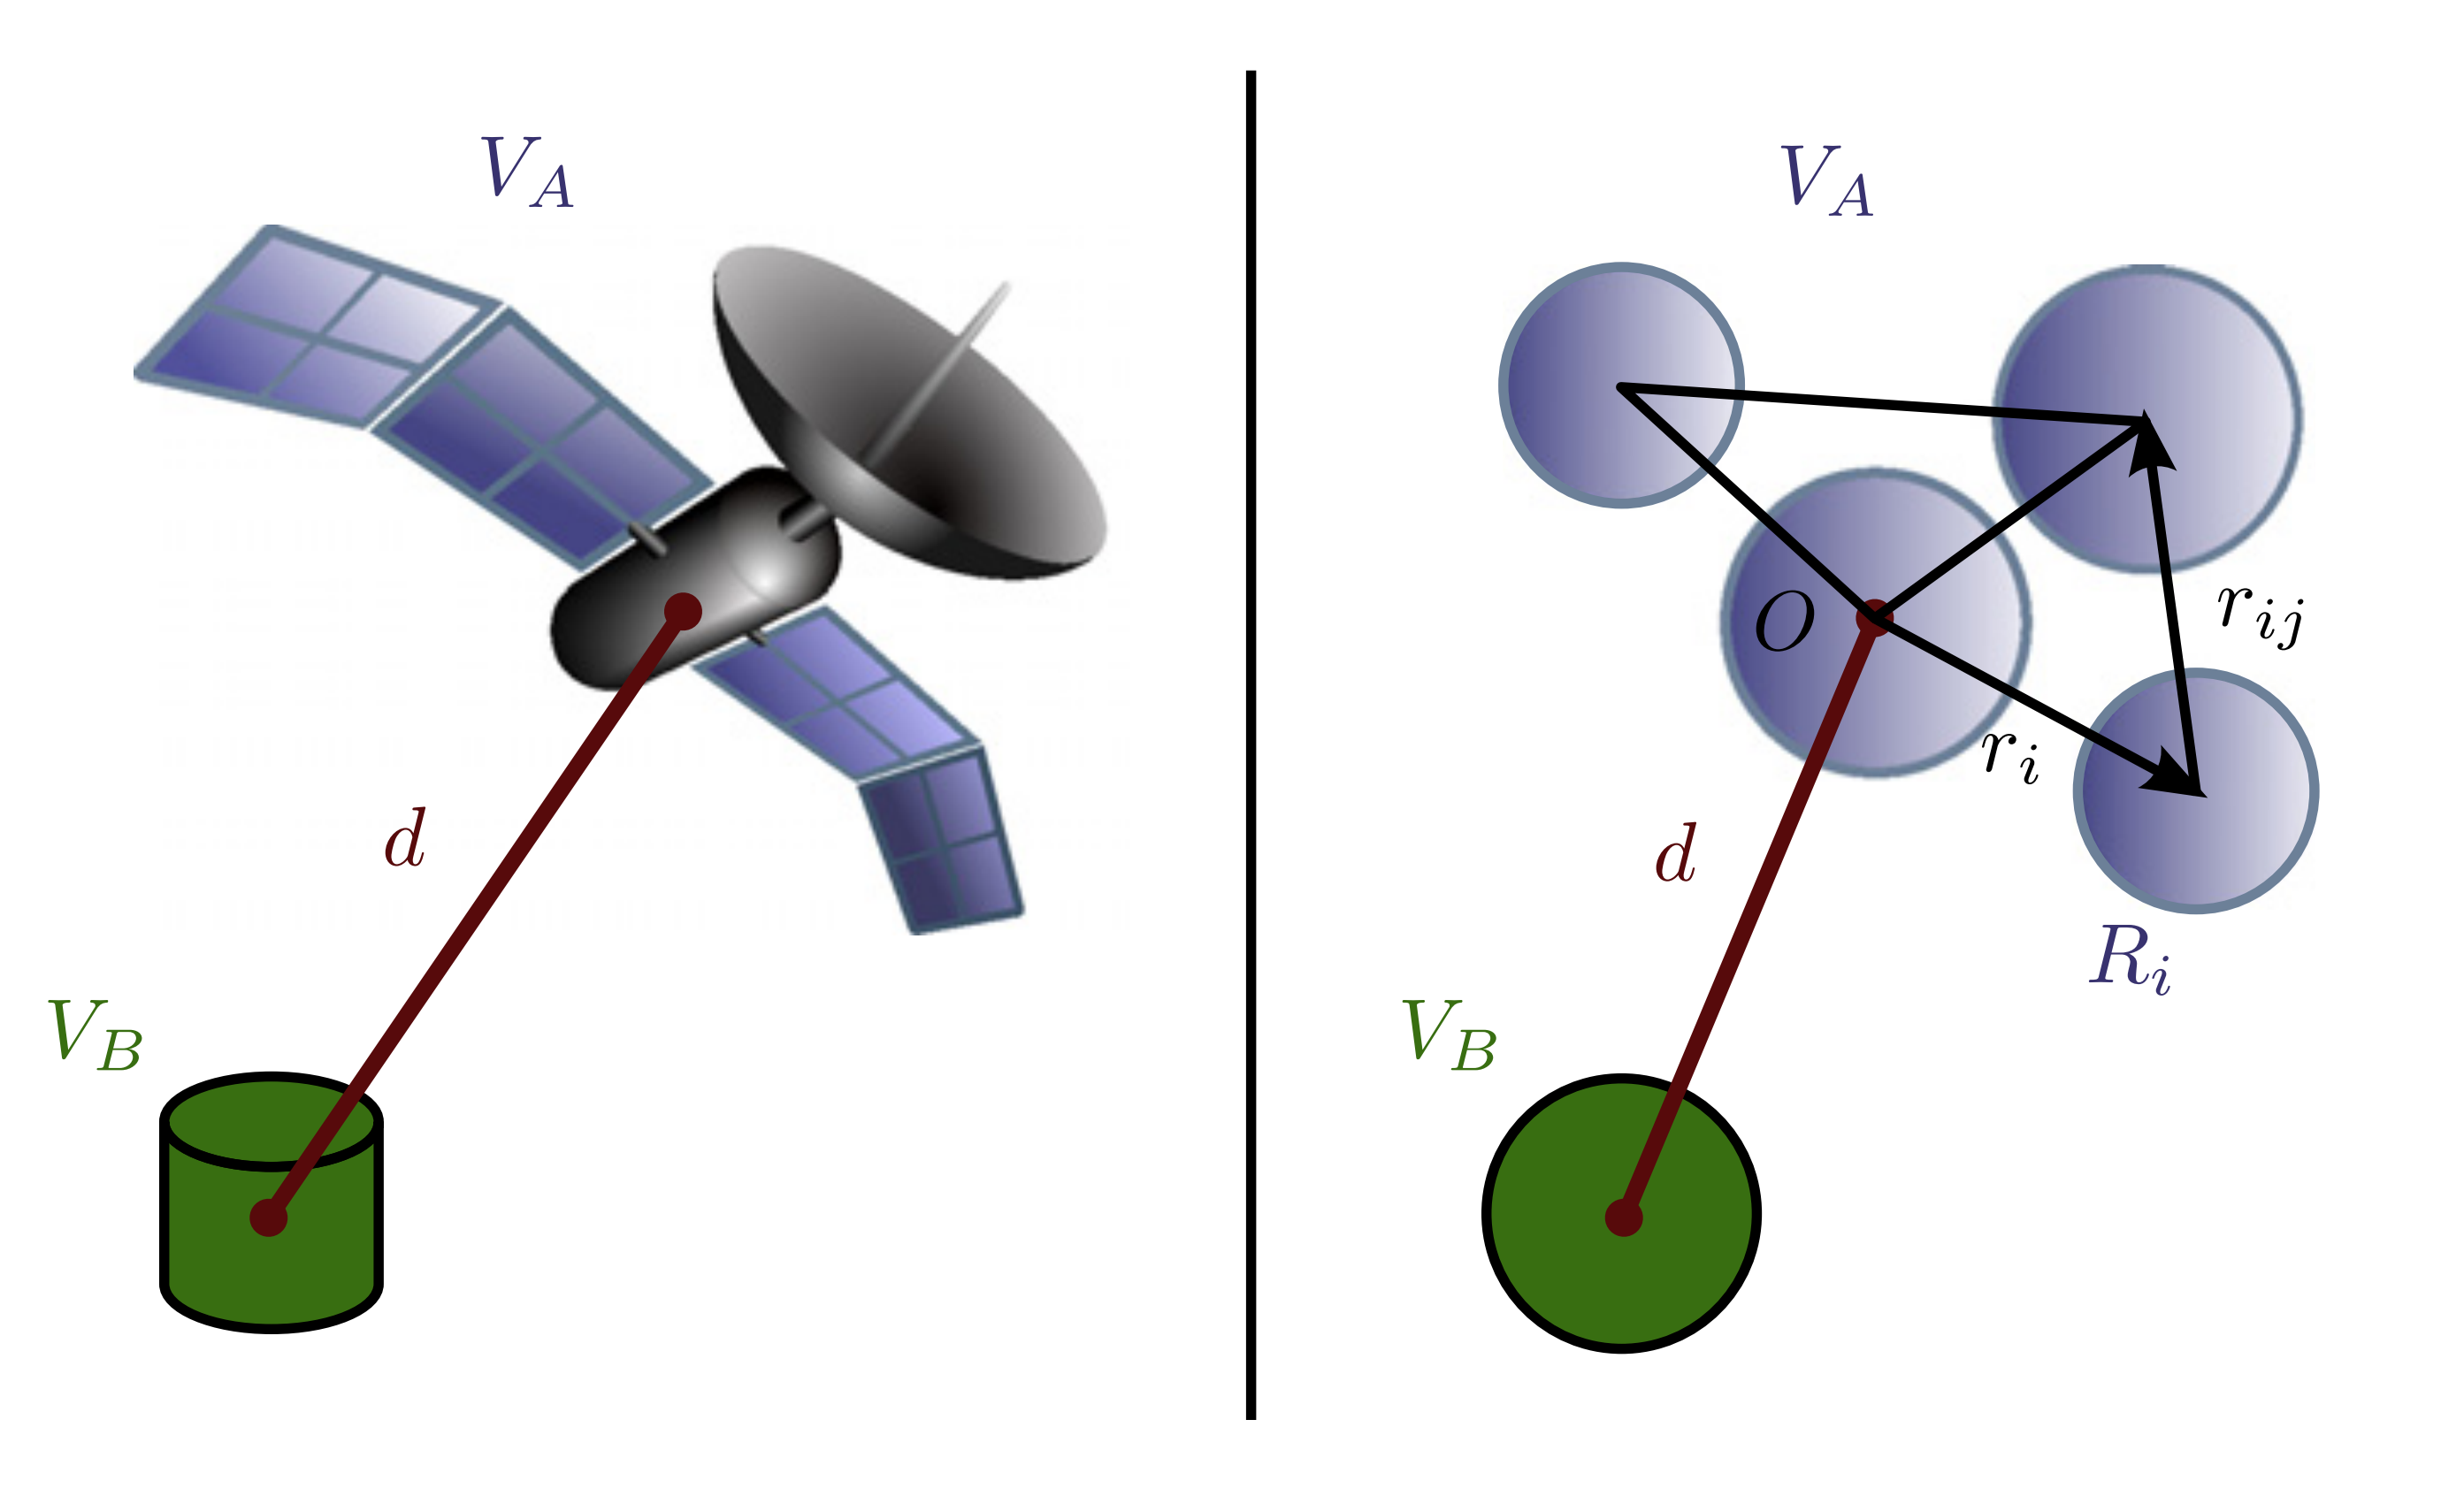
\includegraphics[scale=0.2]{spacecraft_msm.png}}
	\end{figure}
	\footnotesize{\textit{Daan Stevenson and Hanspeter Schaub. Multi-sphere method for modeling electrostatic forces and torques: Advances in Space Research, 51(1):10–20, Jan. 2013.}}
\end{frame}

\begin{frame}
\frametitle{Метод  многих сфер}
\framesubtitle{Вычисление зарядов}
	\begin{equation*}
		\vec{\Phi} = k_c [C_m]^{-1} \vec{q},
	\end{equation*}
	\footnotesize{где $k_c = \frac{1}{4\pi\varepsilon_0} = 8.99 * 10^9 \frac{N*m^2}{C^2}$ – постоянная Кулона, $\vec{\Phi} = [\Phi_A, \Phi_A, \dots, \Phi_A, \Phi_B]^T$ – вектор напряжений, $\vec{q} = [q_1, q_2, \dots, q_n, q_b]^T$ – вектор зарядов, $\Phi_A$ – напряжение каждой сферы тела, $\Phi_B$ – напряжение внешней сферы, $q_i$ – заряд $i$-ой сферы, $C_m$ – матрица ёмкостей.}
	
	\begin{equation*}
		[C_m]^{-1} = 
		\begin{pmatrix}
			1/R_1	&	1/r_{1,2}	&	\dots		&	1/r_{1,n}	&	1/r_{1,B} \\
			1/r_{1,2}	&	1/R_1	&	\dots		&	\vdots		&	\vdots \\
			\vdots		&	\ddots		&	\ddots	&	\vdots		&	\vdots \\
			1/r_{n,1}	&	\dots			&	\dots		&	1/R_n	&	1/r_{n,B} \\
			1/r_{B,1}	&	\dots			&	\dots		&	1/r_{B,n}	&	1/R_B
		\end{pmatrix},
	\end{equation*}
	\footnotesize{где $\vec{r}_{i,B} = \vec{d} - \vec{r}_i$.}
\end{frame}

\begin{frame}
\frametitle{Моделирование движения КА вокруг центра масс с помощью метода многих сфер}
\framesubtitle{Замена КА набором сфер}
	\begin{figure}[H]
		\center{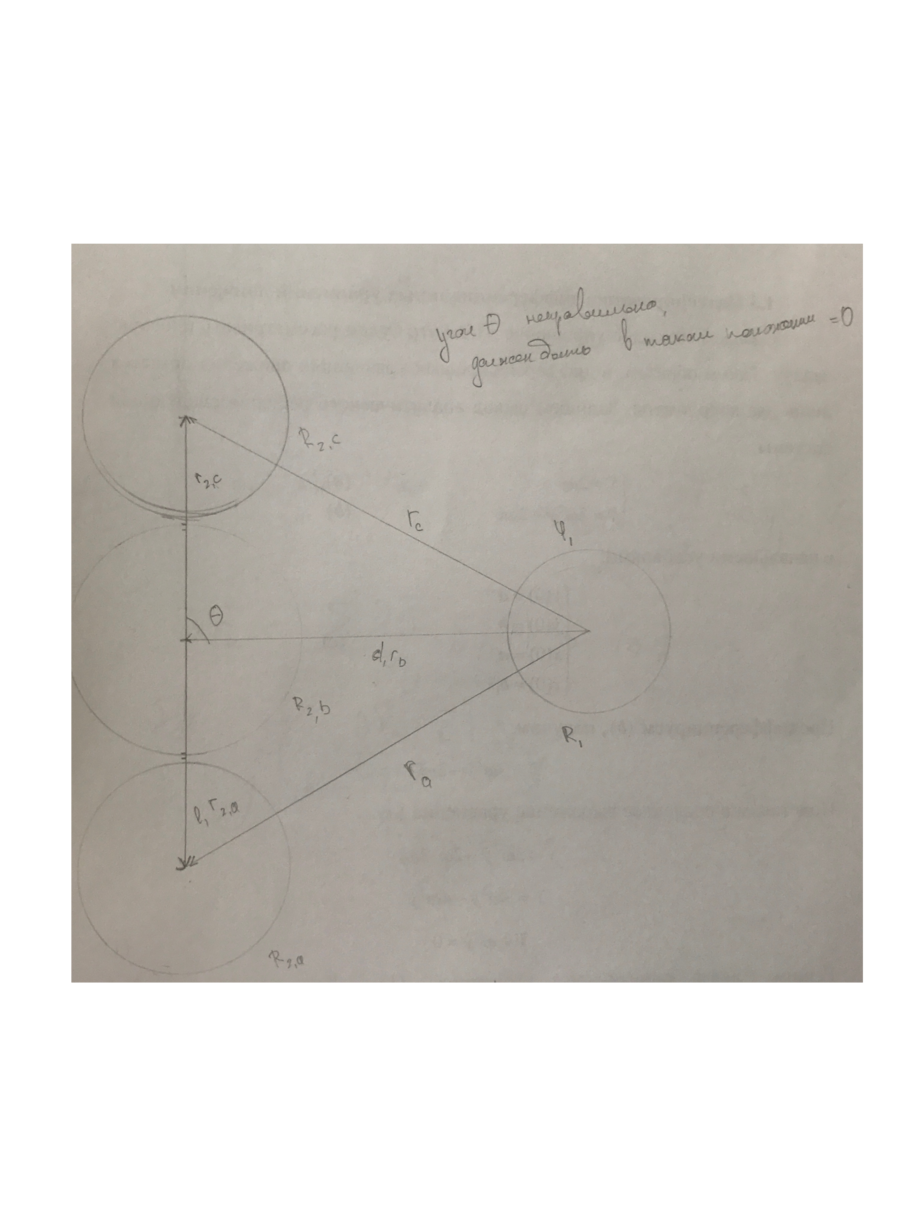
\includegraphics[scale=0.3]{3sph.png}}
	\end{figure}
\end{frame}

\begin{frame}
\frametitle{Моделирование движения КА вокруг центра масс с помощью метода многих сфер}
\framesubtitle{Уравнения движения}
\begin{columns}[onlytextwidth]
	\begin{column}{0.5\textwidth}
	\begin{equation*}
		[C_m]^{-1} = 
		\begin{pmatrix}
			1/R_1	&	1/r_a	&	1/r_b	&	1/r_c\\
			1/r_a	&	1/R_{2a}	&	1/l		&	1/2l\\
			1/r_b	&	1/l		&	1/R_{2b}	&	1/l\\
			1/r_c	&	1/2l		&	1/l		&	1/R_{2c}
		\end{pmatrix},
	\end{equation*}	
	\begin{equation*}
		T = \frac{J \left(\frac{d \theta (t)}{dt}\right)^2}{2},
	\end{equation*}
	\begin{equation*}
		Q_\theta = \frac{\partial \vec{r}_{ba}}{\partial \theta(t)} \cdot F_{2a} + \frac{\partial \vec{r}_{bc}}{\partial \theta(t)} \cdot F_{2c},
	\end{equation*}
	\end{column}
	\begin{column}{0.5\textwidth}
	\begin{equation*}
		\begin{pmatrix}
			q_1\\
			q_{2a}\\
			q_{2b}\\
			q_{2c}
		\end{pmatrix}
		= k_c C_m 
		\begin{pmatrix}
			-\phi\\
			\phi\\
			\phi\\
			\phi
		\end{pmatrix},
	\end{equation*}
	\begin{equation*}
		F_{2a} = - \frac{k_c q_1 q_{2a}}{r_a^3}  R_a,
	\end{equation*}
	\begin{equation*}
		F_{2c} = - \frac{k_c q_1 q_{2c}}{r_c^3} R_c,
	\end{equation*}
	\end{column}
\end{columns}
\begin{center}
$S_a = - k_c q_1 q_{2a}$ и $S_c = - k_c q_1 q_{2c}$.
\end{center}
\end{frame}

\begin{frame}
\frametitle{Моделирование движения КА вокруг центра масс с помощью метода многих сфер}
\framesubtitle{Параметры моделирования}
\begin{columns}[onlytextwidth]
	\begin{column}{0.5\textwidth}
		$\phi = 20000$В,\\$R_1 = 0.5$м,\\$R_{2a} = R_{2c} = 0.59$м,\\$R_{2b} = 0.65$м,\\$l = 1.5$м,
	\end{column}
	\begin{column}{0.5\textwidth}
		$d = 15$м,\\$J = 1000$кг$\cdot$м${}^2$,\\
		$\theta(0) = 1$,\\
		$\theta'(0) = 0.$	
	\end{column}
\end{columns}
\end{frame}

\begin{frame}
\frametitle{Моделирование движения КА вокруг центра масс с помощью метода многих сфер}
\framesubtitle{Результаты моделирования для $d = 20$м и $d = 10$м}
\begin{columns}[onlytextwidth]
	\begin{column}{0.5\textwidth}
		\begin{figure}[H]
			\center{\includegraphics[scale=0.2]{msm_theta_d=20.png}}
		\end{figure}
		\begin{figure}[H]
			\center{\includegraphics[scale=0.2]{msm_flow_d=20.png}}
		\end{figure}	
		\begin{center}
			\footnotesize{$d = 20$м}
		\end{center}
	\end{column}
	\begin{column}{0.5\textwidth}
		\begin{figure}[H]
			\center{\includegraphics[scale=0.2]{msm_theta_d=10.png}}
		\end{figure}
		\begin{figure}[H]
			\center{\includegraphics[scale=0.2]{msm_flow_d=10.png}}
		\end{figure}	
		\begin{center}
			\footnotesize{$d = 10$м}
		\end{center}
	\end{column}
\end{columns}
\end{frame}

\begin{frame}
\frametitle{Моделирование движения КА вокруг центра масс с помощью метода многих сфер}
\framesubtitle{Результаты моделирования для $d = 5$м и $d = 1.8$м}
\begin{columns}[onlytextwidth]
	\begin{column}{0.5\textwidth}
		\begin{figure}[H]
			\center{\includegraphics[scale=0.2]{msm_theta_d=5.png}}
		\end{figure}
		\begin{figure}[H]
			\center{\includegraphics[scale=0.2]{msm_flow_d=5.png}}
		\end{figure}	
		\begin{center}
			\footnotesize{$d = 5$м}
		\end{center}
	\end{column}
	\begin{column}{0.5\textwidth}
		\begin{figure}[H]
			\center{\includegraphics[scale=0.2]{{msm_theta_d=1.8}.png}}
		\end{figure}
		\begin{figure}[H]
			\center{\includegraphics[scale=0.2]{{msm_flow_d=1.8}.png}}
		\end{figure}	
		\begin{center}
			\footnotesize{$d = 1.8$м}
		\end{center}
	\end{column}
\end{columns}
\end{frame}

\begin{frame}
\frametitle{Моделирование движения двух КА как двух материальных точек}
\framesubtitle{Замена космических аппаратов двумя материальными точками}
\begin{columns}[onlytextwidth]
	\begin{column}{0.5\textwidth}
	\begin{figure}[H]
		\center{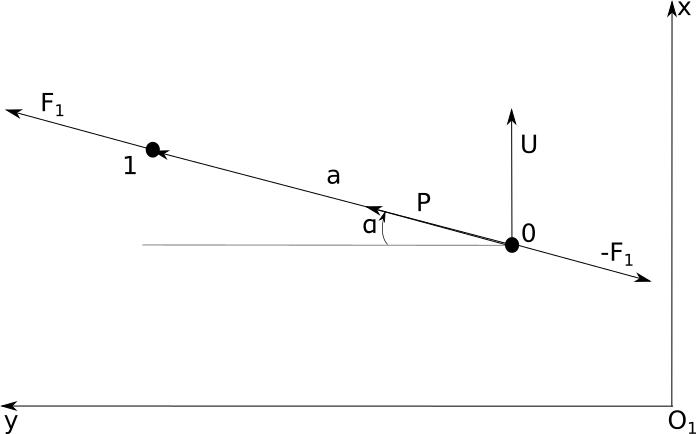
\includegraphics[scale=0.3]{2sph.png}}
	\end{figure}
	\end{column}
	\begin{column}{0.5\textwidth}
		\begin{equation*}
			T = m_0 \frac{\norm{\vec{v}_0}^2}{2} + m_1 \frac{\norm{\vec{v}_1}^2}{2},
		\end{equation*}
		\begin{equation*}
			\vec{F}_1 = \frac{k_c q_0 q_1}{a^3}\vec{A},
		\end{equation*}
		\begin{equation*}
			\vec{F}_0 = \vec{P} - \vec{F}_1,
		\end{equation*}
		\begin{equation*}
			\begin{pmatrix}
				q_x \\
				q_y \\
				q_a \\
				q_\alpha \\
			\end{pmatrix} 
			=
			\begin{pmatrix}
				x \\
				y \\
				a \\
				\alpha \\
			\end{pmatrix},
		\end{equation*}
		\begin{equation*}
			Q_j = \frac{\partial r_0}{\partial q_j} \cdot F_0 + \frac{\partial r_1}{\partial q_j} \cdot F_1.
		\end{equation*}
	\end{column}
\end{columns}
\end{frame}

\begin{frame}
\frametitle{Моделирование движения двух КА как двух материальных точек}
\framesubtitle{Параметры моделирования}
\begin{columns}[onlytextwidth]
	\begin{column}{0.5\textwidth}
		$m_0 = 200$кг,\\$m_1=1000$кг,\\$p=0.2$H,\\$k_c q_0 q_1=8.3 * 10^{-3}$,\\
		$x(0) = 0$, \\
		$y(0) = 0$, \\
		$a(0) = 5.4$, \\
	\end{column}
	\begin{column}{0.5\textwidth}
		$\alpha(0) = 0$,\\
		$x'(0) = 0$, \\
		$y'(0) = 0$, \\
		$a'(0) = 0$, \\
		$\alpha'(0) = 0.01$.
	\end{column}
\end{columns}
\end{frame}

\begin{frame}
\frametitle{Моделирование движения двух КА как двух материальных точек}
\framesubtitle{Результаты моделирования}
\begin{columns}[onlytextwidth]
	\begin{column}{0.5\textwidth}
		\begin{figure}[H]
			\center{\includegraphics[scale=0.2]{2sph_no_u_a.png}}
		\end{figure}
		\scriptsize{Зависимость координаты $a$ от времени $t$}
		\begin{figure}[H]
			\center{\includegraphics[scale=0.2]{2sph_no_u_alpha.png}}
		\end{figure} 
		\scriptsize{Зависимость координаты $\alpha$ от времени $t$}
	\end{column}
	\begin{column}{0.5\textwidth}
		\begin{figure}[H]
			\center{\includegraphics[scale=0.2]{2sph_no_u_x.png}}
		\end{figure} 
		\scriptsize{Зависимость координаты $x$ от времени $t$}
		\begin{figure}[H]
			\center{\includegraphics[scale=0.2]{2sph_no_u_y.png}}
		\end{figure} 
		\scriptsize{Зависимость координаты $y$ от времени $t$}
	\end{column}
\end{columns}
\end{frame}

\begin{frame}
\frametitle{Моделирование движения двух КА как двух материальных точек}
\framesubtitle{Управление по $\alpha$}
		\begin{equation*}
			\vec{U} = 
			\begin{pmatrix}
				\cos \alpha \left(k_\alpha \sin \alpha + k_{\alpha t}\alpha'\right)\\
				\sin \alpha \left(k_\alpha \sin \alpha + k_{\alpha t}\alpha'\right)
			\end{pmatrix}
		\end{equation*}
		
		\begin{equation*}
			\vec{F}_0 = \vec{P} - \vec{F}_1 + \vec{U}.
		\end{equation*}
\end{frame}

\begin{frame}
\frametitle{Моделирование движения двух КА как двух материальных точек}
\framesubtitle{Результаты моделирования с управлением по $\alpha$ при $k_\alpha = -5$ и $k_{\alpha t} = -2$}
\begin{columns}[onlytextwidth]
	\begin{column}{0.5\textwidth}
		\begin{figure}[H]
			\center{\includegraphics[scale=0.2]{2sph_alpha_u_a.png}}
		\end{figure}
		\scriptsize{Зависимость координаты $a$ от времени $t$}
		\begin{figure}[H]
			\center{\includegraphics[scale=0.2]{2sph_alpha_u_alpha.png}}
		\end{figure} 
		\scriptsize{Зависимость координаты $\alpha$ от времени $t$}
	\end{column}
	\begin{column}{0.5\textwidth}
		\begin{figure}[H]
			\center{\includegraphics[scale=0.2]{2sph_alpha_u_x.png}}
		\end{figure} 
		\scriptsize{Зависимость координаты $x$ от времени $t$}
		\begin{figure}[H]
			\center{\includegraphics[scale=0.2]{2sph_alpha_u_y.png}}
		\end{figure} 
		\scriptsize{Зависимость координаты $y$ от времени $t$}
	\end{column}
\end{columns}
\end{frame}

\begin{frame}
\frametitle{Моделирование движения двух КА как двух материальных точек}
\framesubtitle{Управление по $\alpha$ и $\theta$}
		\begin{equation*}
			\vec{U} = 
			\begin{pmatrix}
				\cos \alpha \left(k_\alpha \sin \alpha + k_{\alpha t}\alpha' + k_x x + x_{xt} x'\right)\\
				\sin \alpha \left(k_\alpha \sin \alpha + k_{\alpha t}\alpha' + k_x x + x_{xt} x'\right)
			\end{pmatrix}
		\end{equation*}
\end{frame}

\begin{frame}
\frametitle{Моделирование движения двух КА как двух материальных точек}
\framesubtitle{Результаты моделирования с управлением по $\alpha$ и $\theta$ при $k_x = 0.1$ и $k_{x t} = 0.1$}
\begin{columns}[onlytextwidth]
	\begin{column}{0.5\textwidth}
		\begin{figure}[H]
			\center{\includegraphics[scale=0.2]{2sph_full_u_a.png}}
		\end{figure}
		\scriptsize{Зависимость координаты $a$ от времени $t$}
		\begin{figure}[H]
			\center{\includegraphics[scale=0.2]{2sph_full_u_alpha.png}}
		\end{figure} 
		\scriptsize{Зависимость координаты $\alpha$ от времени $t$}
	\end{column}
	\begin{column}{0.5\textwidth}
		\begin{figure}[H]
			\center{\includegraphics[scale=0.2]{2sph_full_u_x.png}}
		\end{figure} 
		\scriptsize{Зависимость координаты $x$ от времени $t$}
		\begin{figure}[H]
			\center{\includegraphics[scale=0.2]{2sph_full_u_y.png}}
		\end{figure} 
		\scriptsize{Зависимость координаты $y$ от времени $t$}
	\end{column}
\end{columns}
\end{frame}

\begin{frame}
\frametitle{Моделирование движения пассивного и активного КА}
\framesubtitle{Движение пассивного КА и активного КА по методу многих сфер}
	\begin{figure}[H]
		\center{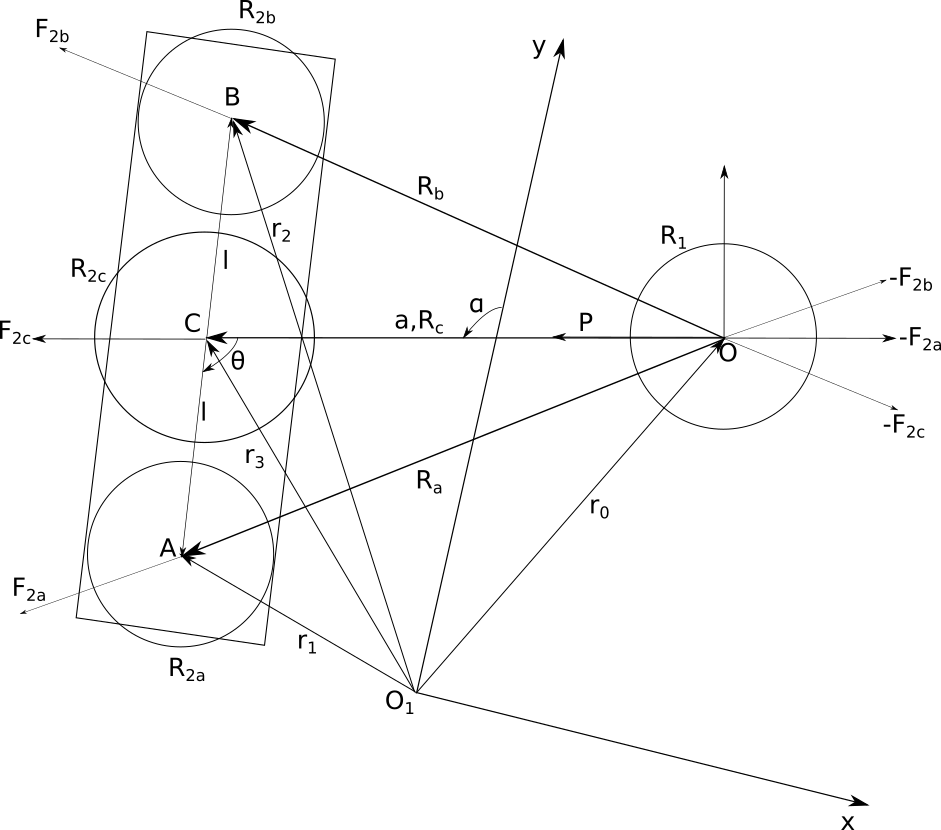
\includegraphics[scale=0.3]{2sph_msm.png}}
	\end{figure}
\end{frame}


\begin{frame}
\frametitle{Моделирование движения пассивного и активного КА}
\framesubtitle{Уравнения движения}
\begin{columns}[onlytextwidth]
	\begin{column}{0.5\textwidth}
	\begin{equation*}
		T = m_0 \frac{\norm{\vec{v}_0}^2}{2} + m_1 \frac{\norm{\vec{v}_1}^2}{2} + \frac{J\left(\frac{d\theta}{dt}\right)^2}{2},
	\end{equation*}	
	\begin{equation*}
			(q_x,q_y,q_a,q_\alpha,q_\theta)^T=(x,y,a,\alpha,\theta)^T,
	\end{equation*}
	\begin{equation*}
		Q_j = \frac{\partial r_0}{\partial q_j} \cdot F_0 + \frac{\partial r_1}{\partial q_j} \cdot F_1 +\frac{\partial r_2}{\partial q_j} \cdot F_2 +\frac{\partial r_3}{\partial q_j} \cdot F_3,
	\end{equation*}
	\begin{equation*}
		\vec{F}_1 = -\frac{k_c q_1 q_{2a}}{r_a^3}\vec{R}_a,
	\end{equation*}
	\begin{equation*}
		\vec{F}_2 = -\frac{k_c q_1 q_{2b}}{r_b^3}\vec{R}_b,
	\end{equation*}
	\begin{equation*}
		\vec{F}_3 = -\frac{k_c q_1 q_{2c}}{r_c^3}\vec{R}_c,
	\end{equation*}
	\begin{equation*}
		\vec{F}_0 = \vec{P} - (\vec{F}_1 + \vec{F}_2 + \vec{F}_3) + \vec{U},
	\end{equation*}
	\end{column}
	\begin{column}{0.5\textwidth}
	\begin{equation*}
		\begin{cases}
			x(0) = 0, \\
			y(0) = 0, \\
			a(0) = 5.4, \\
			\alpha(0) = 0,\\
			\theta(0) = 0.4,\\
			x'(0) = 0, \\
			y'(0) = 0, \\
			a'(0) = 0, \\
			\alpha'(0) = 0.01\\
			\theta'(0) = 0.
		\end{cases}
	\end{equation*}
	\end{column}
\end{columns}
\end{frame}

\begin{frame}
\frametitle{Заключение}
В работе построены новые математические моделей движения указанных космических систем и получены новые результаты, подтверждающих возможность увода космических объектов путем толканий при использовании электростатических сил. Найдены новые законы управления космической системой, предназначенной для увода космического мусора.

На основе полученных математических моделей	 можно уже в настоящее время строить наземные стенды для 2D моделирования указанной системы, а в будущем эти результаты помогут реализовать и летный эксперимент в космосе.
\end{frame}

\begin{frame}
	\begin{center}
		Спасибо за внимание!
	\end{center}
\end{frame}
\end{document}